\chapter{Partial derivative} \label{ch6ch}

Partial derivative studies the effect of a small deviation of one particular independent variable on the multivariable function. It is similar with the normal derivative in many ways, but also has its unique characteristics.

In Section \ref{ch6sec:motivatingexp}, a motivating example is given to illustrate the motivation of introducing partial derivative. In Section \ref{ch6sec:partialtotalderivative}, the definition of partial derivative is given. In Sections \ref{ch6sec:gradient} and \ref{ch6sec:jacobianmatrix}, two very important and commonly used tool derived from partial derivative, namely gradient and Jacobian matrix, are introduced respectively.

\section{A Motivating Example} \label{ch6sec:motivatingexp}

Consider the following motivating example where $y=f(x_1, x_2)$ is a multivariable function with $2$ inputs.

\begin{shortbox}
\Boxhead{A Motivating Example}

Consider
\begin{eqnarray}
    y &=& 2x_1^2 + x_2^2 + 2x_1x_2. \label{ch6eq:motivatingexample}
\end{eqnarray}

Q1: Let $x_2 = 1$ be a constant. Derive $y$ as a function of $x_1$, and calculate its derivative with respect to $x_1$. Similarly, let $x_1 = 1$ be a constant and derive $y$ as a function of $x_2$, and calculate its derivative with respect to $x_2$.

Q2: At $(x_1, x_2) = (1, 1)$, consider small vibrations $\Delta x_1$ and $\Delta x_2$. Approximate $\Delta y$ as a function of $\Delta x_1$ and $\Delta x_2$ using differentiation.

Q3: Find such $x_1$ and $x_2$ that $y$ is minimized.

\end{shortbox}

Equation \eqref{ch6eq:motivatingexample} can be plot in 3-D as Fig. \ref{ch6fig_motivatingexp}.
\begin{figure}
	\centering
	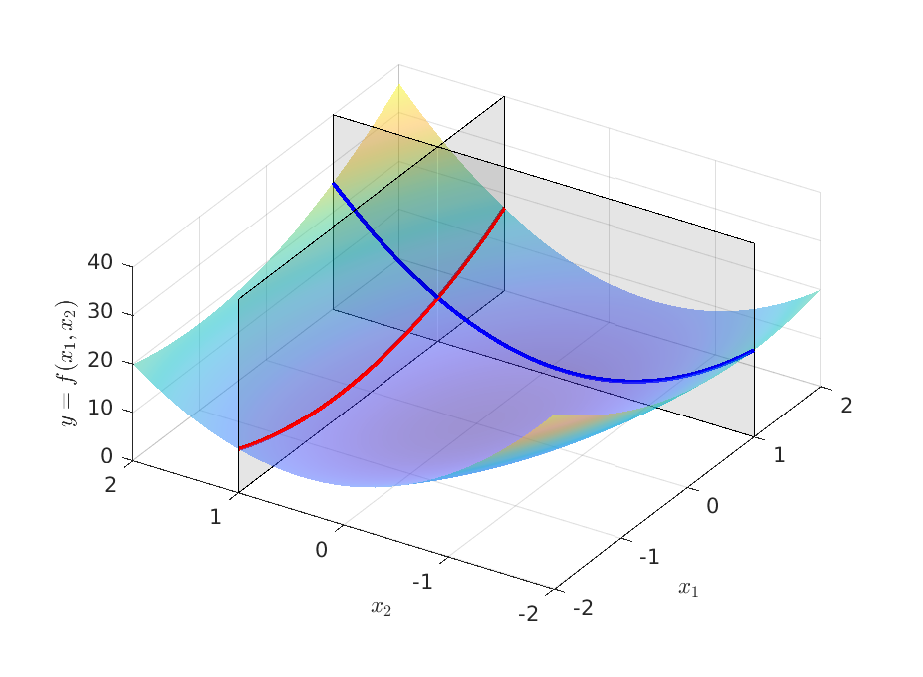
\includegraphics[width=250pt]{chapters/chapter6/figures/fig_motivatingexp.eps}
	\caption{Plot of function $y=f(x_1, x_2)$ in 3-D.} \label{ch6fig_motivatingexp}
\end{figure}

Let $x_2=1$ be constant. Equation \eqref{ch6eq:motivatingexample} becomes
\begin{eqnarray}
	y = f(x_1, 1) = 2x_1^2 + 2x_1 + 1, \nonumber
\end{eqnarray}
which is given by the intersection of  curved surface (equation \eqref{ch6eq:motivatingexample}) and the vertical flat ($x_2=1$) given by the red solid line in Fig. \ref{ch6fig_motivatingexp}. Its derivative with respect to $x_1$ can be easily obtained as
\begin{eqnarray}
	\dfrac{d}{dx_1}f(x_1,1) &=& 4x_1 + 2. \label{ch6eq:motivatingexpdx1}
\end{eqnarray}

Similarly, at $x_1 = 1$, \eqref{ch6eq:motivatingexample} becomes
\begin{eqnarray}
	y = f(1, x_2) = x_2^2 + 2x_2 + 2, \nonumber
\end{eqnarray}
which is given by the blue solid line in Fig. \ref{ch6fig_motivatingexp}. Its derivative with respect to $x_2$ is
\begin{eqnarray}
	\dfrac{d}{dx_2}f(1,x_2) &=& 2x_2 + 2. \label{ch6eq:motivatingexpdx2}
\end{eqnarray}

Consider small vibrations $\Delta x_1$ and $\Delta x_2$. Firstly, let $x_2$ remain constant and only apply $\Delta x_1$ on $y = f(1,1)$. In this case,
\begin{eqnarray}
	\Delta y = f(1+\Delta x_1, 1) - f(1, 1) \approx \dfrac{d}{dx_1}f(x_1,1) \Delta x_1, \label{ch6eq:partialdifx1}
\end{eqnarray}
where $\dfrac{d}{dx_1}f(x_1,1)$ is given in \eqref{ch6eq:motivatingexpdx1}.

On top of \eqref{ch6eq:partialdifx1}, consider vibration $\Delta x_2$. The derivative of function $f(1+\Delta x_1, x_2)$ with respect to $x_2$ depends on $\Delta x_1$ and it is generally unknown without specifying $\Delta x_1$. However, since \eqref{ch6eq:motivatingexample} is continuous and ``smooth'' (Notice that ``smooth'' has specific definition in mathematics. Here, just take its literal meaning: it is perfectly polished without any edges or spikes.), we can intuitively understand that when $\Delta x_1$ is small, $\frac{d}{dx_2}f(1+\Delta x_1, x_2) \approx \frac{d}{dx_2}f(1, x_2)$, and $\frac{d}{dx_2}f(1+\Delta x_1, x_2) \rightarrow \frac{d}{dx_2}f(1, x_2)$ as $\Delta x_1 \rightarrow 0$. Thus, we have
\begin{eqnarray}
	\Delta y &=& \left(f(1+\Delta x_1, 1 + \Delta x_2) -  f(1+\Delta x_1, 1)\right) + \left(f(1+\Delta x_1, 1) - f(1, 1)\right) \nonumber \\
	&\approx& \dfrac{d}{dx_2}f(1,x_2) \Delta x_2 + \dfrac{d}{dx_1}f(x_1,1) \Delta x_1. \label{ch6eq:motivatingresult1}
\end{eqnarray}

In \eqref{ch6eq:motivatingresult1}, consider $\Delta x_1 \rightarrow 0$ and $\Delta x_2 \rightarrow 0$. Denote such $\Delta x_1$ and $\Delta x_2$ as $dx_1$ and $dx_2$ respectively, and the associated $\Delta y$ as $dy$. Here ``$d(\cdot)$'' represents the \textit{infinitesimal change}. Equation \eqref{ch6eq:motivatingresult1} then becomes
\begin{eqnarray}
	d y &=& \dfrac{d}{dx_2}f(1,x_2) d x_2 + \dfrac{d}{dx_1}f(x_1,1) d x_1. \label{ch6eq:motivatingresult2}
\end{eqnarray}

Equation \eqref{ch6eq:motivatingresult2} can be extended to more general cases where $(x_1, x_2) = (1, 1)$ is not specified. The terms $\dfrac{d}{dx_1}f(x_1,1)$ and $\dfrac{d}{dx_2}f(1,x_2)$ needs to be changed accordingly. For example, $\dfrac{d}{dx_1}f(x_1,1)$ given by \eqref{ch6eq:motivatingexpdx1} shall be changed to
\begin{eqnarray}
	\left.\dfrac{d}{dx_1}f(x_1,x_2)\right|_{x_2 \textup{~is constant}} &=& 4x_1 + 2x_2 \nonumber
\end{eqnarray}
with $x_2$ being any arbitrary constant.

The denotation $\left.\dfrac{d}{dx_1}f(x_1,x_2)\right|_{x_2 \textup{~is constant}}$ can sometimes become ambiguous if not handled carefully. One of the reasons could be that ``$d(\cdot)$'' is used as infinitesimal change as shown before. In this case both $dx_1$ and $dx_2$ contribute to $df(x_1,x_2)$, but we would want $\dfrac{d}{dx_1}f(x_1,x_2)$ here to reflect the deviation of $f(x_1,x_2)$ caused by $dx_1$ only, and it is not convenient to list down all the other variables and put ``is/are constant'' everywhere in the equation. Therefore, instead of saying $\left.\dfrac{d}{dx_1}f(x_1,x_2)\right|_{x_2 \textup{~is constant}}$, we denote
\begin{eqnarray}
	\dfrac{\partial}{\partial x_1} f(x_1, x_2) &=& 4x_1 + 2x_2. \nonumber
\end{eqnarray}
The operator $\dfrac{\partial}{\partial x}$ is called \textit{partial derivative} (with respect to $x$), often followed by a multivariable function $f(x,y)$ where $x$ is one of its inputs. It is similar to the derivative, but emphasizing that the interested function is multivariable, and the derivative of this function with respect to ONLY ONE variable is being studied (and the rest variables assumed constant). Since $\partial f(x)$ is rarely or never used as the infinitesimal of $f(x)$, it will hopefully be less ambiguous.

The formal definition of partial derivative is given in next Section \ref{ch6sec:partialtotalderivative}.

Equation \eqref{ch6eq:motivatingresult2} for general $(x_1,x_2)$, therefore, becomes
\begin{eqnarray}
	d y &=& \dfrac{\partial}{\partial x_2}f(x_1,x_2) d x_2 + \dfrac{\partial}{\partial x_1}f(x_1,x_2) d x_1. \label{ch6eq:motivatingtotaldiff}
\end{eqnarray}

The minimum $y=f(x_1,x_2)$ and its associated $x_1$ and $x_2$ can be found by rewriting \eqref{ch6eq:motivatingexample} as
\begin{eqnarray}
	y &=& x_1^2 + \left(x_1 + x_2\right)^2. \nonumber
\end{eqnarray}
Therefore, the minimum $y$ is $y=0$, at $x_1 = 0$ and $x_1 + x_2 = 0$, i.e., $x_1 = x_2 = 0$.

This can also be solved using \eqref{ch6eq:motivatingtotaldiff}. At the minimum point of $y$, $\dfrac{\partial}{\partial x_2}f(x_1,x_2)$ and $\dfrac{\partial}{\partial x_1}f(x_1,x_2)$ must be both zero. Otherwise, it is always possible to add/subtract a small $\Delta x_1$ or $\Delta x_2$ to further decrease $y$. Thus, from \eqref{ch6eq:motivatingexample}
\begin{eqnarray}
	\dfrac{\partial}{\partial x_1}f(x_1,x_2) &=& 4x_1 + 2x_2 = 0 \nonumber \\
	\dfrac{\partial}{\partial x_2}f(x_1,x_2) &=& 2x_1 + 2x_1 = 0 \nonumber
\end{eqnarray}
which yields $x_1=x_2=0$.

\section{Partial Derivative} \label{ch6sec:partialtotalderivative}

In the case of single input scalar function $f(x), x \in \mathbb{R}$, there is no point to define partial and total derivative, as the derivative with respect to that single variable by itself is the total derivative.

In the case of multivariable function with multiple inputs, $f(x), x \in \mathbb{R}^{R\times 1}$, the definition partial derivative is given below.

\begin{VF}
	\textbf{Definition of Partial Integral}:
	\\
	\\
	Consider function $y = f(x_1,...,x_n)$ where $y$ is the scalar output and $x = \left[x_1, ..., x_n\right]^T$ is a $n\times 1$ vector input. The partial derivative of $y=f(x)$ with respect to $x_i$ is given by
	\begin{eqnarray}
		\dfrac{\partial}{\partial x_i}f(x) = \lim_{\Delta x_i \rightarrow 0} \dfrac{f(x_1,..., x_i + \Delta x_i,...,x_n)-f(x_1,...,x_n)}{\Delta x_i}, \label{ch6eq:formalpartialderivative}
	\end{eqnarray}
	with $x_1,...,x_{i-1}, x_{i+1},..., x_n$ remaining constant, and only $x_i$ is allowed to vary.
	
\end{VF}

Here is another example to help better understand partial derivative. Consider $z=f(x, y)$ a multivariable function of both inputs $x$, $y$ as follows
\begin{eqnarray}
	z = f(x,y) = x^2 + \textup{sin}(y), \label{ch6eq:partialdiffchainexp1}
\end{eqnarray}
where $y = g(x)$ is a single input function of $x$ as follows
\begin{eqnarray}
	y = g(x) = e^x. \label{ch6eq:partialdiffchainexp2}
\end{eqnarray}

Apparently, the value of $z$ ultimately depends on $x$ alone, but in the intermediate calculation, $z$ depends on both $x$ and $y$. The calculation flow is visualized in Fig. \ref{ch6fig_chainexp}.

\begin{figure}
	\centering
	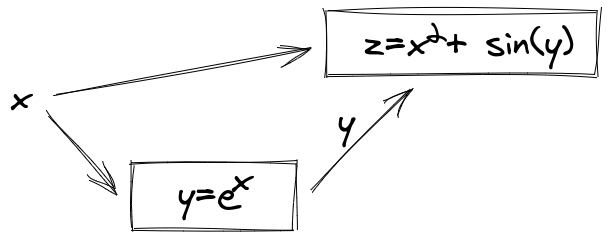
\includegraphics[width=200pt]{chapters/chapter6/figures/chainexp.png}
	\caption{The calculation of $z$ using $x$ and $y$.} \label{ch6fig_chainexp}
\end{figure}

In this case, the total derivative $\dfrac{d}{dx}f(x, y)$ can be expressed as follows
\begin{eqnarray}
	\dfrac{d}{dx}f(x, y) &=& \dfrac{\partial}{\partial x} f(x, y) + \dfrac{\partial}{\partial y}f(x, y) \dfrac{d}{dx}y. \label{ch6eq:partialvstotal}
\end{eqnarray}
where in this example,
\begin{eqnarray}
	\dfrac{\partial}{\partial x} f(x, y) &=& 2x \nonumber \\
	\dfrac{\partial}{\partial y} f(x, y) &=& \textup{cos}(y) \nonumber \\
	\dfrac{d}{dx}y &=& e^x \nonumber
\end{eqnarray}
and finally
\begin{eqnarray}
	\dfrac{d}{dx}f(x, y) &=& 2x + \textup{cos}(e^x)e^x \nonumber
\end{eqnarray}

Sometimes \eqref{ch6eq:partialvstotal} is rewritten as follows
\begin{eqnarray}
	df(x, y) &=& \dfrac{\partial}{\partial x} f(x, y) dx + \dfrac{\partial}{\partial y}f(x, y) dy \nonumber \\
	dy &=& \left(\dfrac{d}{dx}y\right) dx \nonumber
\end{eqnarray}
where $d(\cdot)$ represents the infinitesimal change of a variable.

Equation \eqref{ch6eq:partialvstotal} serves as a good example to show the relationship and difference between the total derivative $\dfrac{d}{dx}f(x, y)$ and the partial derivative $\dfrac{\partial}{\partial x} f(x, y)$. When calculating total derivative, all variables that would affect the value of the function must be taken into consideration, while when calculating partial derivative, only one input variable is studied, with the rest variables remaining constant.

For a function with $1$ output and $n$ inputs, sometimes it is convenient to put the partial derivative to each input in a vector. For example, for $y=f(x)$ where $x = \left[x_1,...,x_n\right]^T$, denote
\begin{eqnarray}
	\dfrac{\partial}{\partial x}f(x) = \left[\begin{array}{ccc}
	\dfrac{\partial}{\partial x_1}f(x) &
	\ldots &
	\dfrac{\partial}{\partial x_n}f(x)
	\end{array}\right] \label{ch6eq:scalarbyvector}
\end{eqnarray}
as the \textit{scalar-by-vector derivative}. Notice that \eqref{ch6eq:scalarbyvector} is usually given as a row vector. In some research papers the result is given as a column vector, i.e. the transpose of \eqref{ch6eq:scalarbyvector}.

For a function with $m$ outputs and $1$ input $y=f(x)$ where $y = \left[y_1,...,y_m\right]^T = \left[f_1(x),...,f_m(x)\right]^T$, its \textit{vector-by-scalar derivative} is given by
\begin{eqnarray}
	\dfrac{\partial}{\partial x}f(x) &=& \left[\begin{array}{c}
	\dfrac{\partial}{\partial x}f_1(x) \\
	\vdots \\
	\dfrac{\partial}{\partial x}f_m(x)
	\end{array}\right]. \label{ch6eq:vectorbyscalar}
\end{eqnarray}

And finally for a function with $m$ outputs and $n$ inputs $y=f(x)$ where $y = \left[y_1,...,y_m\right]^T = \left[f_1(x),...,f_m(x)\right]^T$ and $x = \left[x_1,...,x_n\right]^T$, the \textit{vector-by-vector} derivative is given by
\begin{eqnarray}
	\dfrac{\partial}{\partial x}f(x) &=& \left[\begin{array}{ccc}
	\dfrac{\partial}{\partial x_1}f_1(x) & \ldots & \dfrac{\partial}{\partial x_n}f_1(x) \\
	\vdots & \ddots & \vdots \\
	\dfrac{\partial}{\partial x_1}f_m(x) & \ldots & \dfrac{\partial}{\partial x_n}f_m(x) \\
	\end{array}\right]. \label{ch6eq:vectorbyvector}
\end{eqnarray}

Partial derivative and the above equations \eqref{ch6eq:scalarbyvector}, \eqref{ch6eq:vectorbyscalar} and \eqref{ch6eq:vectorbyvector} have many applications. Two of those most popular use cases are \textit{gradient} and \textit{Jacobian matrix}. Since they are so important and widely used, it is worth especially introducing them in specific Sections \ref{ch6sec:gradient} and \ref{ch6sec:jacobianmatrix}.

\section{Gradient} \label{ch6sec:gradient}

For a scalar-valued multivariable function $y=f(x)$ where $y$ is a scalar and $x$ is a vector $x = \left[\begin{array}{ccc}
                                                                               x_1 & \ldots & x_n
                                                                             \end{array}\right]^T \in \mathbb{R}^n$, the gradient studies the ``direction'' of $\Delta x$ in $\mathbb{R}^n$ space that causes $y$ to increase/decrease the fastest.

The gradient of such function $f(x)$ is a vector function of $x$, denoted by $\nabla f(x)$. Notice that $\nabla f(x) \in \mathbb{R}^n$ is a vector in the same space with $x$, since it indicates a ``direction'' of $x$.

Section \ref{ch6subsec:gradientmotivatingexp} gives a motivating example of gradient, and Section \ref{ch6subsec:gradientdef} gives its formal definition.

\subsection{Motivating Example} \label{ch6subsec:gradientmotivatingexp}

The following motivating example helps to illustrate the calculation and use case of gradient.

\begin{shortbox}
\Boxhead{A Motivating Example}

Consider the following function $y=f(x)$ where $x = [x_1,x_2]^T$ is a vector and
\begin{eqnarray}
    y = f(x) = 2\textup{sin}(x_1) + \textup{sin}\left(\dfrac{x_1}{2} + \pi\right) + \textup{sin}(2x_2) \label{ch6eq:gradientexp_hill}
\end{eqnarray}
where $x_1\in[-3,3]$ and $x_2\in[-2,2]$. The 3-D plot and the contour line of the function are given in Figs \ref{ch6fig:gradientexp_3d} and \ref{ch6fig:gradientexp_contour} respectively.

Consider initial point $x^0 = [x_1^0, x_2^0]^T = [1,0]^T$. Let $x$ deviate a little bit from $x^0$ to get $x^1 = [x_1^1, x_2^1]^T = [x_1^0 + \Delta x_1^0, x_2^0 + \Delta x_2^0]^T$. The objective is to find such $\Delta x^0 = [\Delta x_1^0, \Delta x_2^0]^T$ to hopefully get $f(x^1)$ as large as possible.

\end{shortbox}

\begin{figure}
	\centering
	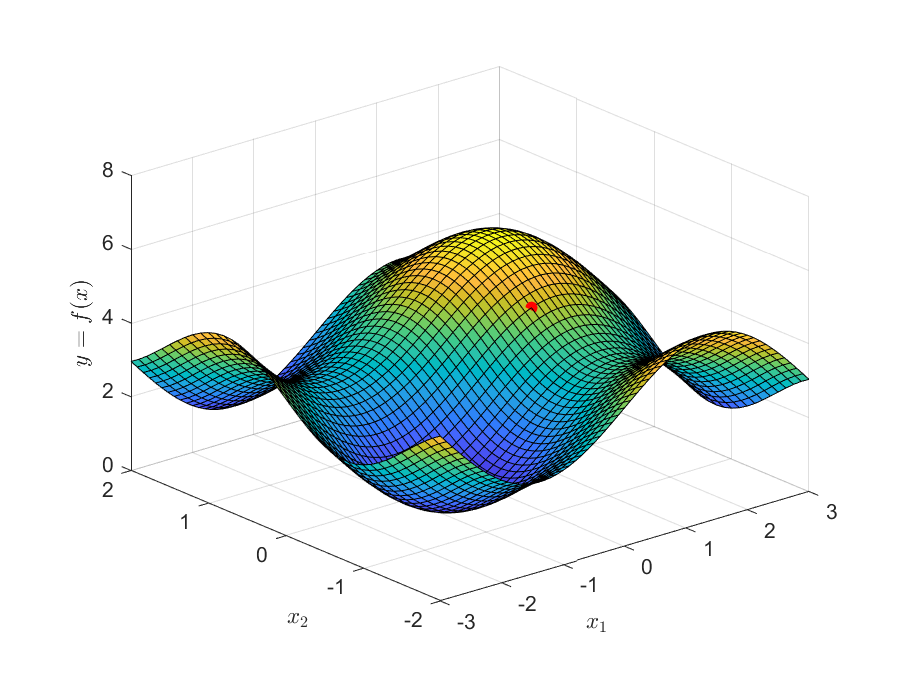
\includegraphics[width=250pt]{chapters/chapter6/figures/gradientexp_3d.eps}
	\caption{Plot of $y=f(x_1, x_2)$ in 3-D.} \label{ch6fig:gradientexp_3d}
\end{figure}
\begin{figure}
	\centering
	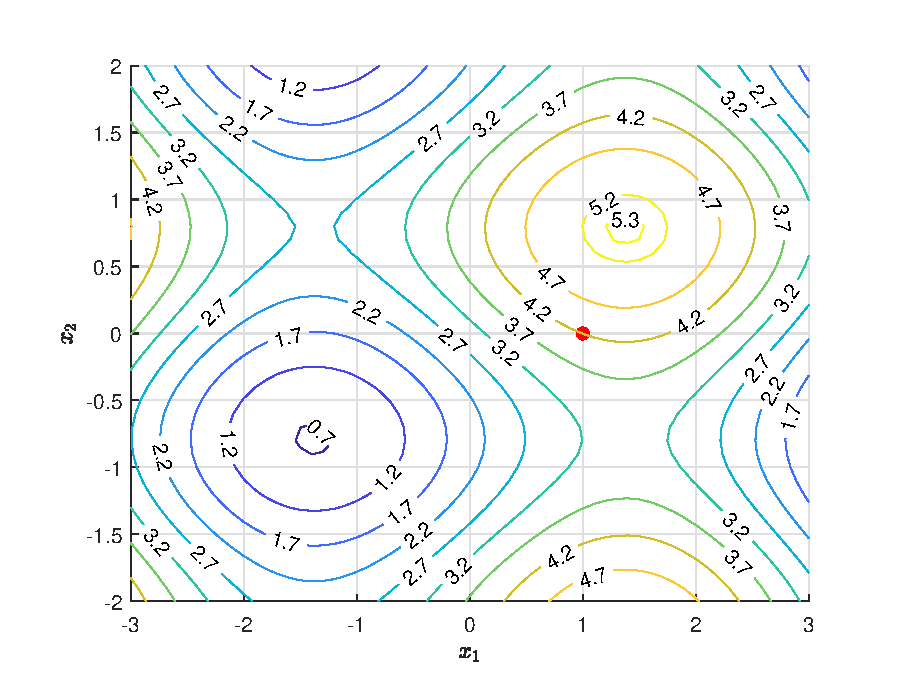
\includegraphics[width=250pt]{chapters/chapter6/figures/gradientexp_contour.eps}
	\caption{Contour line of $y=f(x_1, x_2)$.} \label{ch6fig:gradientexp_contour}
\end{figure}

Notice that $\Delta x^0$ can be interpreted as a vector that points to the ``direction'' of $x$ where $y$ increases the fastest. An intuitive way is to find the tangent plane to the surface given by \eqref{ch6eq:gradientexp_hill} at $x^0=[1,0]^T$, and let $\Delta x^0$ be the direction where it climbs up the tangent plane the fastest.

From space analytic geometry, we know that a pair of unparalleled vector on the tangent plane can uniquely define the plane, and such pair of vector is not difficult to find, as
\begin{eqnarray}
 \vec{v}_1 &=& \left(\begin{array}{ccc}
                       1, & 0, & \left.\dfrac{\partial f(x)}{\partial x_1}\right|_{x=x^0}
                     \end{array}\right) \label{ch6eq:gradientexp_v1} \\
 \vec{v}_2 &=& \left(\begin{array}{ccc}
                       0, & 1, & \left.\dfrac{\partial f(x)}{\partial x_2}\right|_{x=x^0}
                     \end{array}\right) \label{ch6eq:gradientexp_v2}
\end{eqnarray}
must be such a pair of vector. This is because \eqref{ch6eq:gradientexp_v1}, as shown by the red dashed line in Fig. \ref{ch6fig:gradientexp_3d2}, is the tangent of the 2-D intersection of $y=f(x)$ and $x_2 = x_2^0$ shown by the red solid line, therefore must be tangent to the original 3-D surface $y=f(x)$ at $x^0$. The same applies to \eqref{ch6eq:gradientexp_v2}. The tangent plane derived from these two vectors is shown in Fig. \ref{ch6fig:gradientexp_3d3}.

\begin{figure}
	\centering
	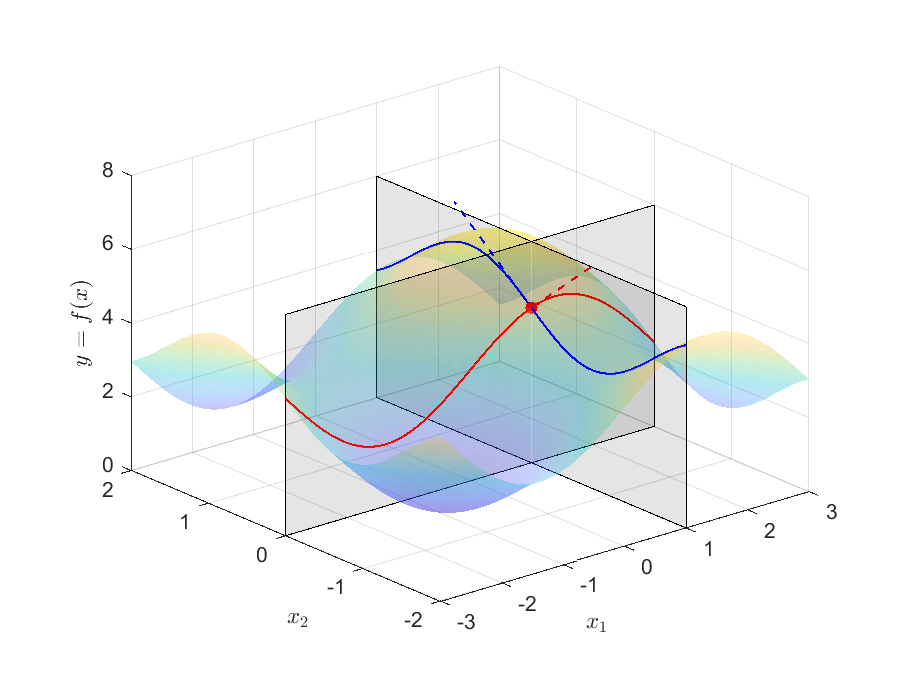
\includegraphics[width=250pt]{chapters/chapter6/figures/gradientexp_3d2.eps}
	\caption{Plot of vectors given by \eqref{ch6eq:gradientexp_v1} and \eqref{ch6eq:gradientexp_v2}.} \label{ch6fig:gradientexp_3d2}
\end{figure}

\begin{figure}
	\centering
	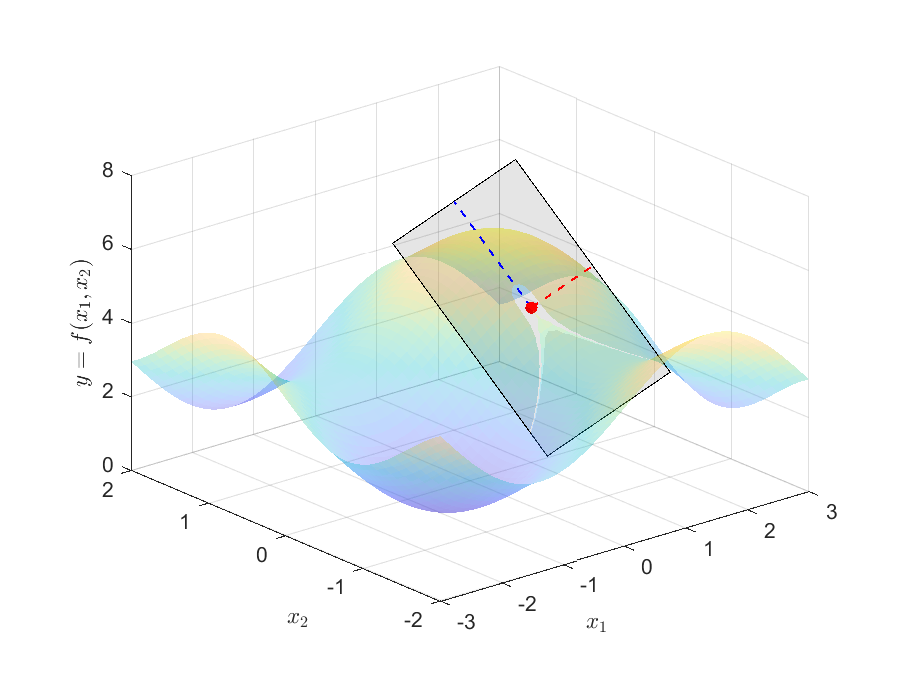
\includegraphics[width=250pt]{chapters/chapter6/figures/gradientexp_3d3.eps}
	\caption{Formulation of the tangent plane from vectors given by \eqref{ch6eq:gradientexp_v1} and \eqref{ch6eq:gradientexp_v2}.} \label{ch6fig:gradientexp_3d3}
\end{figure}

The next step is to find a vector $\vec{v}$ on the tangent plane along which $y$ increases the fastest. For convenience, we will do a plane transformation to the tangent plane so that it crosses the origin $(0,0,0)$. This can be done by mapping $\left(x_1^k,x_2^k,f(x_1^k,x_2^k)\right)$ to $(0,0,0)$. The vector $\vec{v}$ must fulfill the following two conditions: (a) it must be on the tangent plane; (b) it must be perpendicular to the intersection line of the tangent plane and the $y=0$ plane.

Consider (a). Since the vector is on the tangent plan, it can be represented as a linear combination of \eqref{ch6eq:gradientexp_v1} and \eqref{ch6eq:gradientexp_v2} as
\begin{eqnarray}
    \vec{v}&=& \left(\begin{array}{ccc}
              \lambda_1, & \lambda_2, & \lambda_1\left.\dfrac{\partial f(x)}{\partial x_1}\right|_{x=x^0} + \lambda_2\left.\dfrac{\partial f(x)}{\partial x_2}\right|_{x=x^0}
            \end{array} \right) . \label{ch6eq:gradient_v}
\end{eqnarray}

Consider (b). The analytical expression for the tangent plane can be obtained by calculating its normal vector as follows.
\begin{eqnarray}
  \vec{n} &=& \vec{v}_1 \times \vec{v}_2 \nonumber \\
  &=& \left(\begin{array}{ccc}
              -\left.\dfrac{\partial f(x)}{\partial x_1}\right|_{x=x^0}, & -\left.\dfrac{\partial f(x)}{\partial x_2}\right|_{x=x^0}, & 1
            \end{array}\right) \nonumber
\end{eqnarray}
Therefore, the tangent plan is given by (cross origin $(0,0,0)$)
\begin{eqnarray}
  y &=& \left.\dfrac{\partial f(x)}{\partial x_1}\right|_{x=x^0} x_1 + \left.\dfrac{\partial f(x)}{\partial x_2}\right|_{x=x^0} x_2 \nonumber
\end{eqnarray}
And its intersection with plane $y=0$ is
\begin{eqnarray}
  \left.\dfrac{\partial f(x)}{\partial x_1}\right|_{x=x^0} x_1 + \left.\dfrac{\partial f(x)}{\partial x_2}\right|_{x=x^0} x_2 &=& 0 \label{ch6eq:gradient_intersectline}
\end{eqnarray}
Vector $\vec{v}$ must be perpendicular to \eqref{ch6eq:gradient_intersectline}. The direction of the intersection can be represented by a vecotr. From \eqref{ch6eq:gradient_intersectline}, for example,
\begin{eqnarray}
   \vec{v}_{\textup{ints}} &=& \left(\begin{array}{ccc}
              \left.\dfrac{\partial f(x)}{\partial x_2}\right|_{x=x^0}, & -\left.\dfrac{\partial f(x)}{\partial x_1}\right|_{x=x^0}, & 0
            \end{array}\right), \label{ch6eq:gradient_intersectvector}
\end{eqnarray}
is a good choice. Vector $\vec{v}_{\textup{ints}}$ in \eqref{ch6eq:gradient_intersectvector} is perpendicular to $\vec{v}$ in \eqref{ch6eq:gradient_v}. From \eqref{ch6eq:gradient_v} and \eqref{ch6eq:gradient_intersectvector}, equating $\vec{v} \cdot \vec{v}_{\textup{ints}} = 0$ gives
\begin{eqnarray}
  \lambda_1 \left.\dfrac{\partial f(x)}{\partial x_2}\right|_{x=x^0} &=& \lambda_2 \left.\dfrac{\partial f(x)}{\partial x_1}\right|_{x=x^0} \label{ch6eq:gradient_lambdarestrict}
\end{eqnarray}

Equation \eqref{ch6eq:gradient_lambdarestrict} has infinite number of solutions, resulting in infinite number of $\vec{v}$, all of which point to the same direction. For example, select $\lambda_1 = \left.\dfrac{\partial f(x)}{\partial x_1}\right|_{x=x^0}$, $\lambda_2 = \left.\dfrac{\partial f(x)}{\partial x_2}\right|_{x=x^0}$ as the solution. Substituting $\lambda_1$ and $\lambda_2$ into \eqref{ch6eq:gradient_v} gives
\begin{eqnarray}
  \vec{v} &=& \left(\begin{array}{cc}
              \left.\dfrac{\partial f(x)}{\partial x_1}\right|_{x=x^0}, & \left.\dfrac{\partial f(x)}{\partial x_2}\right|_{x=x^0},
            \end{array} \right. \nonumber \\
            && \left. \left.\dfrac{\partial f(x)}{\partial x_1}\right|_{x=x^0} \left.\dfrac{\partial f(x)}{\partial x_1}\right|_{x=x^0} + \left.\dfrac{\partial f(x)}{\partial x_2}\right|_{x=x^0} \left.\dfrac{\partial f(x)}{\partial x_2}\right|_{x=x^0} \right). \label{ch6eq:gradient_finalv}
\end{eqnarray}

Equation \eqref{ch6eq:gradient_finalv} gives the guidance of the direction from $x^0$ to $x^{1}$ which can hopefully maximize $f(x^1)$. Therefore, $\Delta x^0$ can be obtained as follows.
\begin{eqnarray}
  \Delta x^0 &=& \alpha \left[\begin{array}{c}
                         \left.\dfrac{\partial f(x)}{\partial x_1}\right|_{x=x^0} \\
                         \left.\dfrac{\partial f(x)}{\partial x_2}\right|_{x=x^0}
                       \end{array}\right] \nonumber \\
  &=& \alpha \left.\nabla f(x)\right|_{x=x^0} \label{ch6eq:gradientdeltaxresult}
\end{eqnarray}
where $\alpha > 0$ is an adjustable parameter to determine the progressing rate for each iteration and
\begin{eqnarray}
  \nabla f(x) &=& \left[\begin{array}{c}
                         \dfrac{\partial f(x)}{\partial x_1} \\
                         \dfrac{\partial f(x)}{\partial x_2}
                       \end{array}\right] \label{ch6eq:gradientdef}
\end{eqnarray}
is defined as the \textit{gradient} of $f(x)$, which by itself is a vector function of $x$ that has the same dimension with $x$. In this example, since $x$ is a $2\times 1$ vector, $\nabla f(x)$ is also $2 \times 1$. Substituting \eqref{ch6eq:gradientexp_hill} into \eqref{ch6eq:gradientdef} gives
\begin{eqnarray}
  \nabla f(x) &=& \left[\begin{array}{c}
                         2\textup{cos}(x_1) + \dfrac{1}{2}\textup{cos}\left(\dfrac{x_1}{2}+\pi\right) \\
                         2\textup{cos}(2x_2)
                       \end{array}\right]. \label{ch6eq:gradientresult}
\end{eqnarray}
Substituting $x^0=[1,0]^T$ into \eqref{ch6eq:gradientresult} and \eqref{ch6eq:gradientdeltaxresult} gives
\begin{eqnarray}
  \Delta x^0 &=& \alpha \left[\begin{array}{c}
                         0.6418 \\
                         2
                       \end{array}\right] \nonumber
\end{eqnarray}

The above procedures can be used to iteratively calculate $x^k$ as follows.
\begin{eqnarray}
  \Delta x^k &=& \alpha \left.\nabla f(x)\right|_{x=x^k} \nonumber \\
  x^{k+1} &=& x^k + \Delta x^k \nonumber
\end{eqnarray}
until $\left.\nabla f(x)\right|_{x=x^k} \approx 0$ or $f(x^{k+1})-f(x^k) \approx 0$. Following the same concept, each $f(x^{k+1})$ will be slightly larger than $f(x^k)$ and eventually the maximum value of $f(x)$ and its associated $x$ can be achieved. In this example, calculating $x^1$ to $x^{20}$ gives the following trajectory of $x$ as shown in Figs. \ref{ch6fig:gradientexp_3d4} and \ref{ch6fig:gradientexp_3d5}. The value $\alpha = 0.05$ is used. The maximum $y=5.32$ can be achieved at $x^{20} = [1.32, 0.77]^T$. Note that this is already a practically good approximation to the actual maximum, as shown in Figs. \ref{ch6fig:gradientexp_3d4} and \ref{ch6fig:gradientexp_3d5} To get a even better approximation, consider using smaller $\alpha$ and increase the iteration time.

\begin{figure}
	\centering
	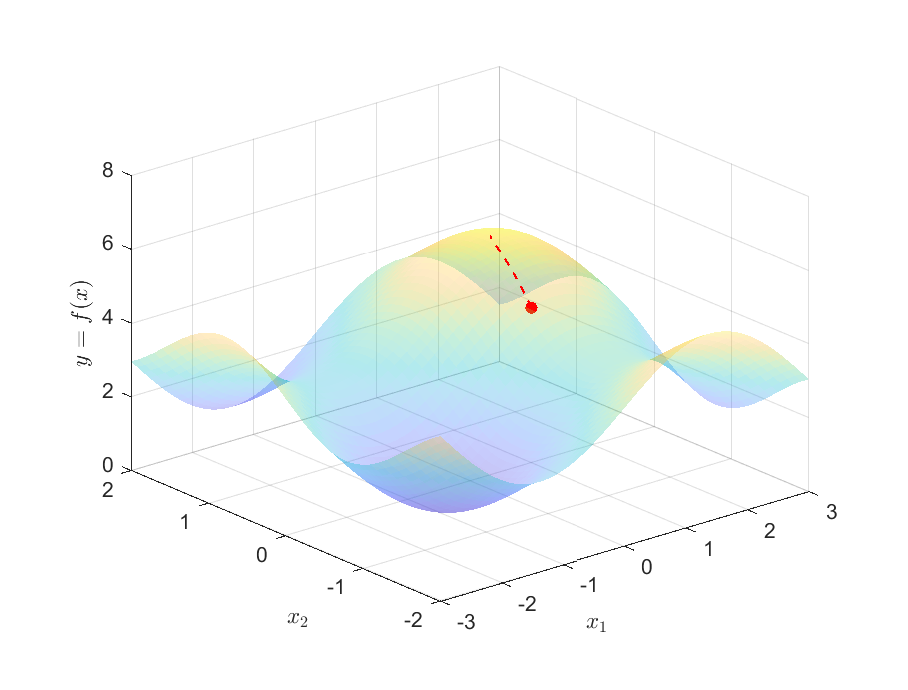
\includegraphics[width=250pt]{chapters/chapter6/figures/gradientexp_3d_trajectory.eps}
	\caption{Trajectory of $x$ until the maximum $y=f(x)$ is achieved.} \label{ch6fig:gradientexp_3d4}
\end{figure}

\begin{figure}
	\centering
	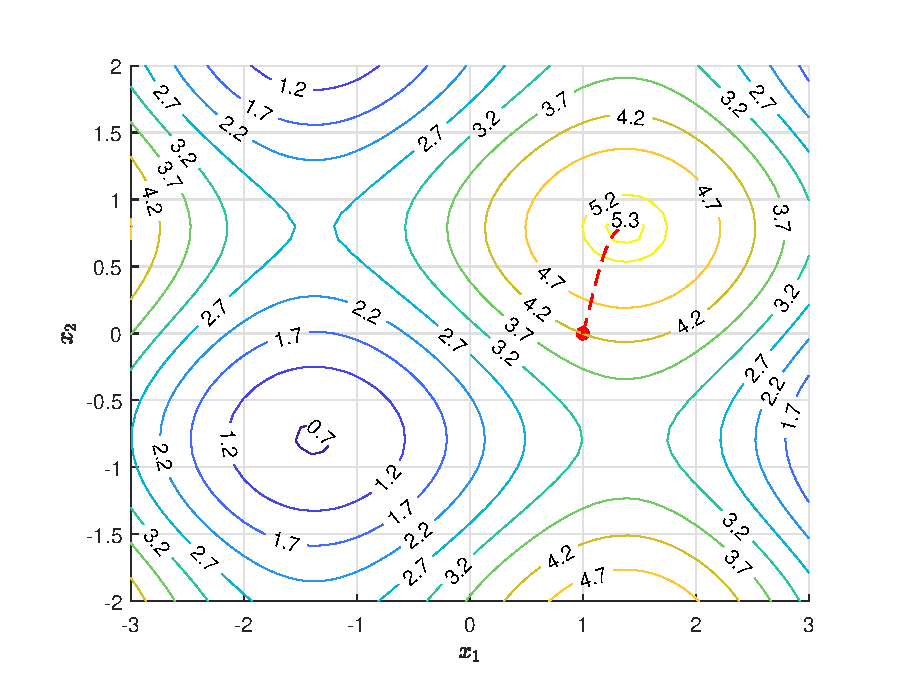
\includegraphics[width=250pt]{chapters/chapter6/figures/gradientexp_contour_trajectory.eps}
	\caption{Trajectory of $x$ until the maximum $y=f(x)$ is achieved on contour line plot.} \label{ch6fig:gradientexp_3d5}
\end{figure}

\subsection{Gradient of a Multivariable Function} \label{ch6subsec:gradientdef}

The gradient of $f(x)$ in \eqref{ch6eq:gradientdef} for the motivating example holds true for general multivariable functions, as long as $f(x)$ is differentiable. The formal definition of gradient is given as follows.

\begin{VF}
	\textbf{Definition of Gradient}:
	\\
	\\
Consider a scalar-valued differentiable function $y=f(x)$ where $x = [x_1,...,x_n]^T \in \mathbb{R}^{n \times 1}$. The gradient of $f(x)$ is a vector function of $x$ denoted by $\nabla f(x) \in \mathbb{R}^{n \times 1}$ as follows. The symbol $\nabla$ is called the \textit{nabla symbol}.
\begin{eqnarray}
  \nabla f(x) &=& \left[\begin{array}{c}
                          \dfrac{\partial}{\partial x_1}f(x) \\
                          \vdots \\
                          \dfrac{\partial}{\partial x_n}f(x)
                        \end{array}\right]. \nonumber
\end{eqnarray}

The gradient of $f(x)$ at point $x=p$ can be calculated by
\begin{eqnarray}
  \nabla f(p) &=& \left.\left[\begin{array}{c}
                         \dfrac{\partial}{\partial x_1}f(x) \\
                          \vdots \\
                          \dfrac{\partial}{\partial x_n}f(x)
                        \end{array}\right]\right|_{x = p}. \nonumber
\end{eqnarray}
which can be interpreted as the direction and rate of fastest increase of $f(x)$ at $x=p$.
	
\end{VF}

In case where the direction and rate of fastest decrease of $f(x)$ is required, $-\nabla f(x)$ can be used. Note that $-\nabla f(x)$ is the direction and rate of fastest increase $-f(x)$.

Do note that local maximum/minimum may become an issue while using gradient-based methods to search for maximum/minimum of a function, depending on the function itself and also the initial point $x_0$ of the iterations.

\section{Jacobian Matrix} \label{ch6sec:jacobianmatrix}

Jacobian matrix is widely used in linear system analysis. For example, it can be used when linearizing a non-linear vector function. The use of Jacobian matrix differs from case to case, thus is not introduced in details here. Only the definition is given as follows.

\begin{VF}
	\textbf{Definition of Jacobian Matrix}:
	\\
	\\
    Consider a vector function $y=f(x)$ where $y = \left[y_1,...,y_m\right]^T \in \mathbb{R}^{m \times 1}$ and $x = [x_1,...,x_n]^T \in \mathbb{R}^{n \times 1}$. The Jacobian matrix of $f(x)$ is an $m \times n$ matrix, usually denoted by $J$ given by
	\begin{eqnarray}
	  J &=& \left[\begin{array}{c}
	                \nabla^T f_1(x) \\
	                \vdots \\
	                \nabla^T f_m(x)
	              \end{array}\right] \nonumber \\
        &=& \left[\begin{array}{ccc}
                    \dfrac{\partial}{\partial x_1}f_1(x) & \ldots & \dfrac{\partial}{\partial x_n}f_1(x) \\
                    \vdots & \ddots & \vdots \\
                    \dfrac{\partial}{\partial x_1}f_m(x) & \ldots & \dfrac{\partial}{\partial x_n}f_m(x)
                  \end{array}\right], \nonumber
	\end{eqnarray}
where $f_i(x)$ is the $i$th element among the $m$ elements in $f(x)$ and $\nabla^T f_i(x)$ is the transpose of $\nabla f_i(x)$.
\end{VF}

Sometimes the characteristics of $J$ reveals insights of function $f(x)$, and can be very helpful in evaluating system performance under particular situations.
